\section{Criterio 5: K-MEANS ISOLATION FOREST}

Dati i contributi di ciascun valore singolare, descritti in (\ref{fj:contributi}), si è scelto di utilizzare il criterio K-Means Isolation Forest.\\
La prima operazione è stata quella di calcolare il logaritmo di ciascun contributo e successivamente dividere i valori in 2 cluster: \textbf{Rumore} e \textbf{Informazione}.\\
Il K-Means però è un apprendimento non supervisionato, dunque non è possibile sapere a priori quale cluster corrisponda a Rumore e quale a Informazione.\\
Poichè nei valori singolari
\begin{equation}
    \sigma_1 >= \sigma_2 >= \sigma_3 >= ... >= \sigma_r>=0
\end{equation}
allora sicuramente il cluster contenente il contributo di $\sigma_1$ sarà quello relativo all'informazione.\\
Una volta identificato tale cluster, si procede a rilevare anomalie mediante l'algoritmo di Isolation Forest.\\

\noindent Il risultato dell'algoritmo ha portato a mantere i primi 225 valori singolari
 \begin{table}[H]
    \centering
    \begin{tabular}{|c|c|c|}
        \hline
        \textbf{Matrice} & \textbf{Righe} & \textbf{Colonne} \\
        \hline
        U\_troncata & 301 & 225 \\
        \hline
        S\_troncata & 225 & 225 \\
        \hline
        V\_troncata & 301 & 225 \\
        \hline
    \end{tabular}
    \caption{Dimensioni matrici troncate}
\end{table}

\begin{table}[H]
    \centering
    \begin{tabular}{|c|c|c|}
        \hline
        \textbf{Norma} & \textbf{Errore assoluto} \\
        \hline
        2 & 141.942286  \\
        \hline
        Frobenius & 723.122392 \\
        \hline
    \end{tabular}
    \caption{Norme ed errori}
\end{table}

\noindent
E' noto inoltre che l'errore assoluto in norma due risulta essere $\sigma_{k+1}$ e in norma Frobenius 
\begin{equation}
    \sqrt{\sum_{i=k+1}^{r}\sigma_i^2}
\end{equation}
 dove k è il numero di valori singolari mantenuti.\\
Per la binarizzazione sono state utilizzate le seguenti soglie:
\begin{itemize}
    \item 0.25
    \item 0.5
    \item 0.75
    \item Soglia automatica calcolata con \textbf{graythresh}
\end{itemize}

\begin{figure}[H]
    \centering
     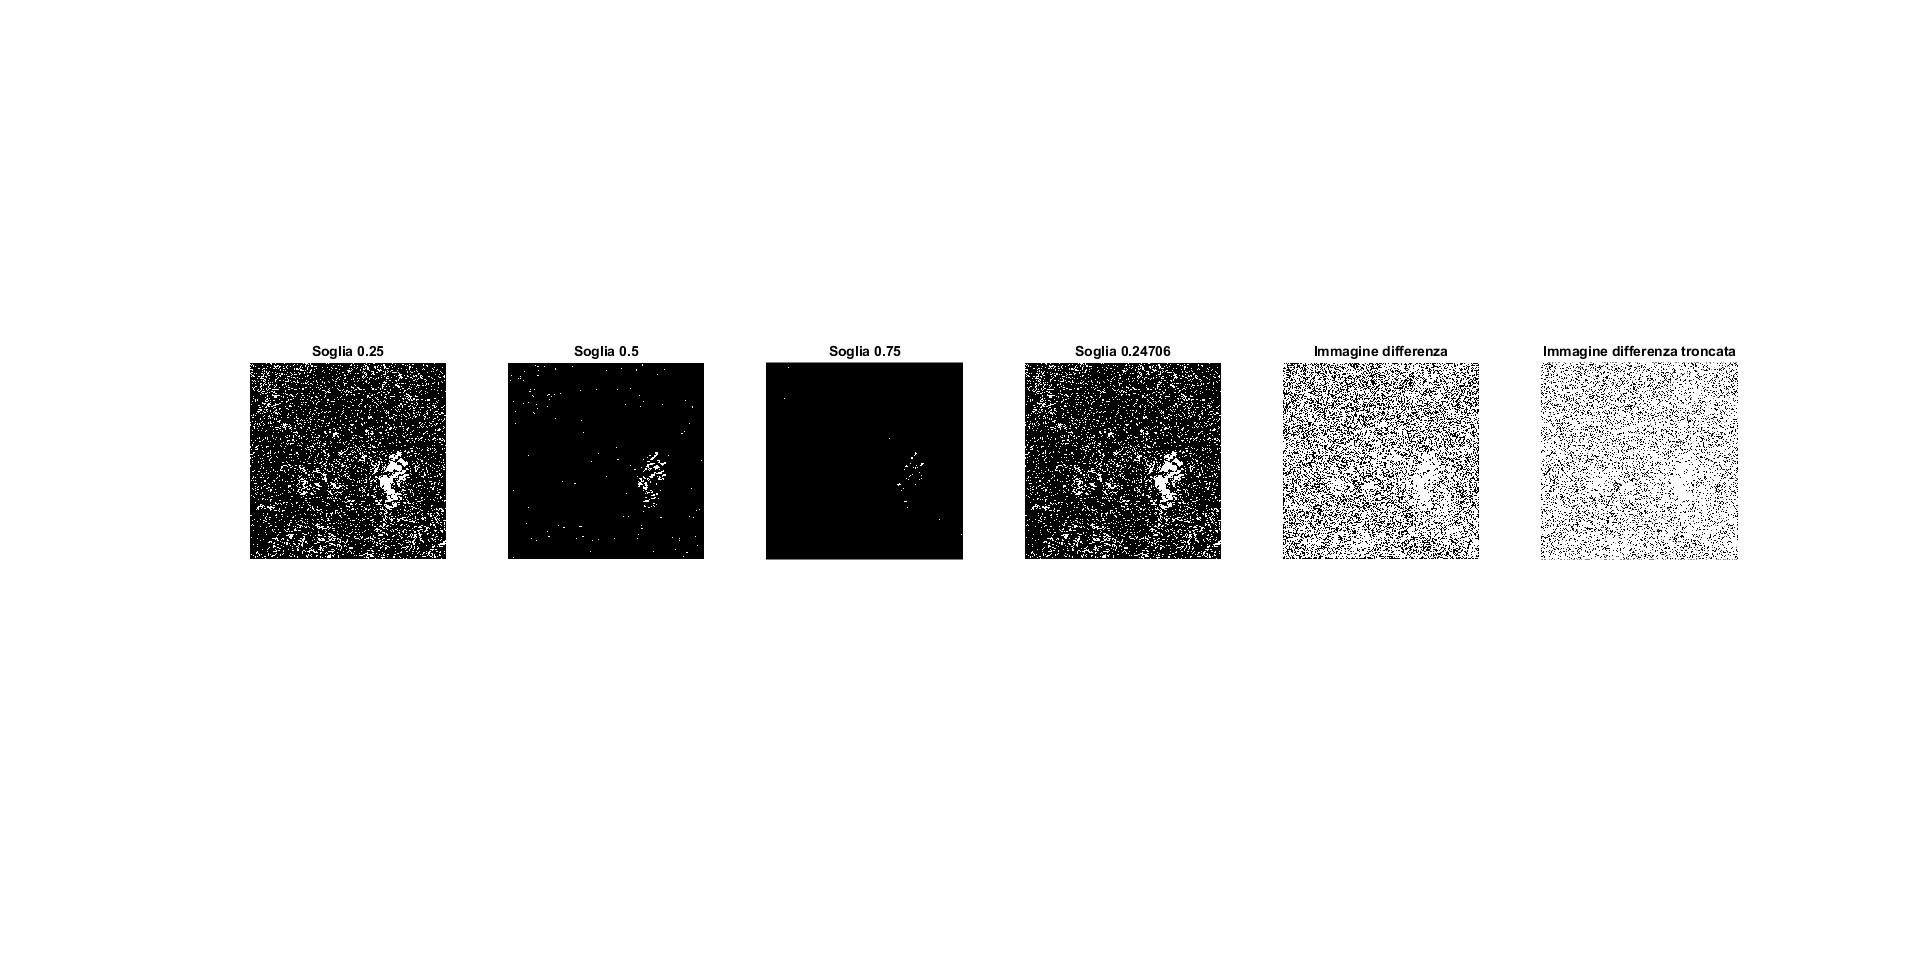
\includegraphics[width=\textwidth]{images/Criterio5.jpg}
    \caption{Immagini binarizzate con criterio 5}
\end{figure}

\noindent Le soglie 0.25 e automatica sono molto simili tra loro e sono "coerenti" sia con l'immagine originale che con quella troncata.

\noindent Per il processo di troncamento sono stati necessari in media circa \textcolor{blue}{\textbf{0.35}} secondi.\\

